\documentclass{ctexart}
\usepackage{graphicx} % Required for inserting images
\usepackage[margin=2.5cm]{geometry}
\usepackage{booktabs}
\usepackage{float}
\usepackage{soulutf8}
\usepackage{enumitem}
\usepackage{pifont}
\usepackage{pgfplots}
\usepackage{longtable}
\pgfplotsset{compat=newest}
\usepackage{tikz}
\usepackage{xcolor} % 用于颜色设置
\usepackage{listings} % 用于代码块
\usepackage{fontspec} % 关键：用于使用系统字体 (XeLaTeX/LuaLaTeX)
% Linux 环境中没有 Windows 宋体时，使用可用的中文衬线字体作为宋体替代
\setCJKmainfont{Noto Serif CJK SC}
\usepackage{authblk}
\usepackage[
    colorlinks=true,      % 使用颜色而非方框
    linkcolor=blue,       % 内部链接颜色
    citecolor=green,      % 引用链接颜色
    urlcolor=red,         % URL 链接颜色
    bookmarks=true,       % 生成 PDF 书签
    bookmarksopen=true,   % 默认展开书签
    pdfstartview=FitH     % 页面宽度适应窗口
]{hyperref}

\sethlcolor{yellow}%设置所需高亮颜色
\usepackage[most]{tcolorbox}
\tcbuselibrary{listings,skins,breakable}
% 页眉页脚
\usepackage{fancyhdr}
\pagestyle{fancy}

% 定义草绿色
\definecolor{grassgreen}{RGB}{124,179,66}
% 补全缺失的浅蓝色定义（防止编译报错）
\definecolor{lightblue}{RGB}{30,144,255} 

% 清空默认
\fancyhf{}
\setlength{\headheight}{14pt}

% 页眉
\fancyhead[L]{\textcolor{lightblue}{\kaishu Computer Vision}}
\fancyhead[R]{\textcolor{lightblue}{\textit{2026.9-2027.1}}}

% 页脚页码居中
\fancyfoot[C]{\textcolor{lightblue}{\thepage}}

% 页眉、页脚线颜色
\renewcommand{\headrulewidth}{1pt}
\renewcommand{\footrulewidth}{1pt}
\renewcommand{\headrule}{\color{blue!30!white}\hrule height 1pt width\headwidth}
\renewcommand{\footrule}{\color{blue!30!white}\hrule height 1pt width\headwidth}
\newtcolorbox{fancybox}[2][blue]{ % 可选颜色参数
  enhanced,
  breakable,
    colback=#1!3!white,
    colframe=#1!18!white,
    boxrule=0.8pt,
    arc=6pt,
    outer arc=6pt,
  left=10pt,right=10pt,top=12pt,bottom=10pt,
  title={\textbf{#2}},
    fonttitle=\bfseries\color{#1!65!black},
  attach boxed title to top left={yshift=-2mm,xshift=5mm},
  boxed title style={
        colback=#1!8!white,
        colframe=#1!18!white,
        boxrule=0.6pt,
        arc=4pt,
  },
    shadow={1.5pt}{-1.5pt}{0pt}{black!10},
}

% 定义一套适合C++的配色方案
\usepackage{tabularx}
\newfontfamily{\consolasfont}{Ubuntu}

\newcommand{\bluecode}[1]{{\color{blue}\consolasfont #1}}
\lstdefinestyle{MyCppStyle}{
    language = C++,
    % 确保这里使用 \consolasfont
    basicstyle = \consolasfont\small, 
    keywordstyle = \color{blue!70!black}, 
    commentstyle = \color{green!50!black}, 
    stringstyle = \color{red!60!black}, 
    numberstyle = \tiny\color{gray}, 
    numbers = left, 
    frame = single, 
    rulecolor = \color{lightgray}, 
    breaklines = true, 
    backgroundcolor = \color{white}, 
    tabsize = 4, 
    showstringspaces = false, 
    xleftmargin = 2em, 
    escapeinside=``,
}
% --- lstdefinestyle HTML 风格定义 ---
\lstdefinestyle{mhtml}{
    language = HTML,
    basicstyle = \consolasfont\small, 
    tagstyle = \color{blue!70!black}\bfseries,
    keywordstyle = \color{purple!80!black},
    commentstyle = \color{green!50!black}\itshape, 
    stringstyle = \color{red!60!black}, 
    numberstyle = \tiny\color{gray}, 
    numbers = left, 
    frame = single, 
    rulecolor = \color{lightgray}, 
    breaklines = true, 
    backgroundcolor = \color{white}, 
    tabsize = 4, 
    showstringspaces = false, 
    xleftmargin = 2em, 
    escapeinside=``,
    morekeywords={als, doctype, html, head, title, meta, link, body, div, span, h1, h2, h3, h4, h5, h6, p, a, img, ul, ol, li, table, tr, th, td, pre, code, script, style},
    morekeywords=[2]{class, id, href, src, rel, type, charset, lang, name, content, style},
    keywordstyle=[2]\color{purple!80!black},
}
\usepackage{hyperref}
\hypersetup{
    colorlinks=true,      
    linkcolor=blue,       
    filecolor=magenta,    
    urlcolor=cyan,        
    pdftitle={我的文档标题}, 
}

% ==================== 正文部分 ====================
\begin{document}

% 开启无页眉页脚模式（针对封面和目录）
\pagestyle{empty}

% ------------------ 美化封面页 ------------------
\begin{titlepage}
    \centering
    % 顶部 TikZ 几何几何装饰条（全宽 bleed 效果）
    \begin{tikzpicture}[remember picture, overlay]
        \fill[blue!50!white] (current page.north west) rectangle ([yshift=-2cm]current page.north east);
        \fill[grassgreen] (current page.north west) ++(0,-2cm) rectangle ([yshift=-2.2cm]current page.north east);
    \end{tikzpicture}
    
    \vspace*{3.5cm}
    
    % 大标题
    {\fontsize{30pt}{36pt}\selectfont\bfseries\color{blue!80!black} 计算机视觉（CV）}\\[0.6em]
    % 副标题或英文标识
    {\fontsize{14pt}{18pt}\selectfont\color{gray}\textsf{Computer Vision}}\\[1cm]
    
    % 居中装饰线
    \centering\makebox[4cm]{\color{grassgreen}\rule{5cm}{1.5pt}}
    
    \vfill
    
    % 使用 tcolorbox 包装的精致作者信息框
    \begin{tcolorbox}[
        enhanced,
        width=0.55\textwidth,
        colback=blue!5!white,
        colframe=blue!5!white,
        boxrule=1.2pt,
        arc=6pt,
        sharp corners=downhill, % 别致的对角切角效果
        shadow={2pt}{-2pt}{0pt}{black!20},
        halign=center,
        valign=center,
        top=15pt, bottom=15pt
    ]
        {\large\bfseries\color{black!80} Author：} {\large\kaishu Simson} \\[0.6em]
        {\large\bfseries\color{black!80} Date：} {\large\kaishu September 2026}
    \end{tcolorbox}
    
    \vfill
    \vspace*{2cm}
    
    % 底部标识
    {\color{gray!80}\small\the\year\ \copyright\ All Rights Reserved.}
\end{titlepage}

\pagestyle{fancy}

\newpage
\tableofcontents
\newpage

% 设置从当前页（正文第一页）开始采用阿拉伯数字编码，并自动重置为第 1 页
\pagenumbering{arabic}

这是计算机视觉（CV）的课堂笔记，笔记参考PPT和课程教材，课堂PPT为英文，尽量写成中文版

\section{Introduction to Computer Vision}

\subsection{Computer Vision Concepts}

``Make computers see.''

\begin{itemize}
\item 输入：光学采样（optical sampling）得到的图像、视频或其他传感器数据。
\item 输出：三维场景表示和重建（3D scene representation and reconstruction），以及物体和场景的语义（semantic）。
\item 目标：将光学输入转换为语义和结构，回答“图像中有什么、在哪里、是什么，以及接下来可能发生什么”。
\end{itemize}

\subsection{History of Computer Vision}

计算机视觉并不是一开始就等同于“识别图片中的物体”。它的发展始终围绕一个核心问题展开：如何把二维图像中的光照、颜色和几何信息，转换为对现实世界中物体、场景和行为的可计算理解。

\begin{enumerate}[label=\arabic*.]
    \item \textbf{萌芽阶段：从成像到图像处理（Image Formation and Image Processing）。}
    摄影术、照相机和光学成像理论为计算机视觉提供了数据来源。计算机出现后，研究者首先关注图像的数字化、去噪、增强、边缘检测（edge detection）和分割（segmentation）等问题。这一时期的重点是回答“图像中有哪些可测量的结构”，而不是直接理解图像内容。

    \item \textbf{早期人工智能阶段：把视觉看作符号推理（Symbolic Reasoning）。}
    20世纪60年代，计算机视觉逐渐成为人工智能（Artificial Intelligence）的研究方向。早期系统尝试从线条、角点和简单几何图形中恢复物体结构，并将视觉结果交给符号系统进行推理。由于真实图像受到遮挡、噪声、光照变化和视角变化的影响，这类依赖人工规则的方法很难扩展到复杂场景。

    \item \textbf{理论化阶段：视觉的多层表示（Hierarchical Representation）。}
    David Marr 提出视觉处理可以分为多个层次：原始图像（primal sketch）、二维半描述（2.5D sketch）以及三维模型（3D model representation）。这一观点强调，视觉不是一次性完成的分类，而是从图像证据逐步构造几何和语义表示（representation）的过程，对后来的三维重建（3D reconstruction）和场景理解（scene understanding）影响深远。

    \item \textbf{经典特征阶段：从人工特征到统计学习（Hand-crafted Features and Statistical Learning）。}
    20世纪90年代至21世纪初，研究者设计了 SIFT（Scale-Invariant Feature Transform）、HOG（Histogram of Oriented Gradients）等局部或区域特征，并结合支持向量机（Support Vector Machine, SVM）等分类器完成识别任务。随后出现的 Viola--Jones 人脸检测器展示了级联分类器（cascade classifier）在实际应用中的效率。这一阶段的典型流程是“特征提取（feature extraction）+ 分类器（classifier）”。

    \item \textbf{深度学习阶段：学习视觉表示（Deep Learning）。}
    大规模数据集、图形处理器（Graphics Processing Unit, GPU）和反向传播（backpropagation）共同推动了卷积神经网络（Convolutional Neural Network, CNN）的发展。2012 年 AlexNet 在 ImageNet 图像分类任务上的成功，使端到端学习（end-to-end learning）成为主流：模型不再完全依赖人工设计特征，而是从数据中联合学习特征和任务目标。目标检测（object detection）、语义分割（semantic segmentation）和实例分割（instance segmentation）也因此获得了显著进步。

    \item \textbf{当前阶段：视觉基础模型（Vision Foundation Models）。}
    近年来，视觉 Transformer（Vision Transformer, ViT）、视觉语言模型（Vision-Language Model, VLM）和多模态大模型（multimodal large model）逐渐成为重要方向。模型可以在大规模图像、文本或视频上进行预训练（pre-training），再通过微调（fine-tuning）或提示学习（prompting）适应下游任务。研究重点也从单一分类任务扩展到图像生成（image generation）、视频理解（video understanding）、三维感知（3D perception）以及具身智能（embodied intelligence）。
\end{enumerate}

\subsection{Overview of Computer Vision}

计算机视觉（Computer Vision, CV）研究如何使计算机从图像和视频中提取信息，并据此完成测量、识别、预测和决策。常用的概括是 ``Make computers see''，但这里的 ``see'' 并不只是把像素读入内存，而是建立从视觉观测（visual observation）到世界模型（world model）的联系。

从信息处理的角度看，计算机视觉通常包含以下三个层次：

\begin{itemize}
    \item \textbf{成像与感知（Imaging and Sensing）：}通过相机（camera）、深度传感器（depth sensor）、激光雷达（LiDAR）等设备获得图像或视频。需要考虑投影模型（projection model）、光照（illumination）、噪声（noise）和相机标定（camera calibration）。
    \item \textbf{表示与理解（Representation and Understanding）：}将像素转换为边缘、关键点（keypoint）、纹理（texture）、物体、姿态（pose）和场景结构等表示，并理解物体之间的空间关系。
    \item \textbf{推理与行动（Inference and Action）：}根据视觉表示完成分类（classification）、检测（detection）、跟踪（tracking）、三维重建（3D reconstruction）、预测（prediction）或控制（control）。
\end{itemize}

按照任务目标，计算机视觉问题可以分为几何视觉（geometric vision）、识别视觉（recognition）、场景理解（scene understanding）和生成视觉（generative vision）等方向。几何视觉关注相机、点、线、平面和三维结构之间的关系；识别视觉关注“图像中有什么”；场景理解进一步回答“它们在哪里、如何相互作用”；生成视觉则根据图像或文本条件生成新的视觉内容。

计算机视觉与图像处理（Image Processing）、计算机图形学（Computer Graphics）、模式识别（Pattern Recognition）和机器学习（Machine Learning）关系密切，但关注点并不完全相同：图像处理主要改变或恢复图像，图形学主要从模型生成图像，而计算机视觉主要从图像反推出物体、场景和行为。实际系统通常会综合使用这些领域的方法。

\subsection{Why Is Computer Vision Hard?}

计算机看到的首先不是“猫”“汽车”或“街道”，而是一组离散的数字。对于一张 RGB 图像（RGB image），每个像素通常由三个颜色通道组成，数值记录的是光在成像平面上的采样结果。计算机需要从例如 $800\times600\times3$ 的数值矩阵中恢复物体、材质、空间位置和正在发生的动作，这中间存在明显的语义鸿沟（semantic gap）。

此外，图像是三维世界在二维平面上的投影（2D projection of the 3D world）。同一个物体在不同视点、光照和距离下可能产生差异很大的图像；反过来，不同的三维场景也可能投影为相同或非常相似的二维图像。因此，从图像恢复真实场景本质上是一个不适定逆问题（ill-posed inverse problem），通常需要引入先验知识（prior knowledge）、物理假设（physical assumptions）或数据驱动的统计规律（data-driven statistics）。

典型困难包括：

\begin{itemize}
    \item \textbf{视点变化（viewpoint variation）：}相机位置或观察方向变化会改变物体的外观、可见表面和投影形状。
    \item \textbf{形变（deformation）：}人体、动物、布料等非刚体（non-rigid object）会改变姿态和局部结构。
    \item \textbf{遮挡（occlusion）：}物体可能被其他物体遮住，系统只能根据不完整的观测推断整体。
    \item \textbf{光照变化（illumination variation）：}阴影、反射、曝光和光源方向会改变像素值，但不一定改变物体本身。
    \item \textbf{运动（motion）：}物体和相机都可能运动，导致运动模糊（motion blur）、目标位移和对应关系变化。
    \item \textbf{局部歧义（local ambiguity）：}局部纹理或轮廓可能对应多个合理解释，例如错觉图形中的边界并不唯一。
    \item \textbf{类内差异与类间相似（intra-class variation and inter-class similarity）：}同一类别的物体可能外观差异很大，而不同类别的物体可能具有相似形状或颜色。
\end{itemize}

因此，视觉系统不仅要完成感知（perception），还要完成测量（measurement）和推理（reasoning）。一个系统能够准确分类，并不意味着它已经恢复了可靠的几何结构；同样，能够测量深度的系统，也未必理解场景中的语义关系。

\subsection{Waves of Computer Vision}

按照研究问题和主要技术路线，计算机视觉的发展可以概括为以下几个阶段：

\begin{enumerate}[label=\arabic*.]
    \item \textbf{启发式视觉（1960--1970，Heuristic Vision）：}研究集中于积木世界（blocks world）、边缘和符号人工智能（symbolic AI）。Larry Roberts 的 Blocks World 试图从二维线条的拓扑结构推断物体的三维结构；1966 年 MIT Summer Vision Project 则体现了早期对视觉问题复杂度的低估。
    \item \textbf{低层视觉（1970--1981，Low-level Vision）：}研究者转向更基础的几何和物理问题，包括阴影形状（shape from shading）、本征图像（intrinsic images）、光度立体（photometric stereo）、双目立体（stereo）、光流（optical flow）和极几何（epipolar geometry）。这些方法说明，视觉理解必须先处理图像形成和空间对应关系。
    \item \textbf{神经网络萌芽（1985--1989，Early Neural Networks）：}反向传播算法（backpropagation）使基于梯度的表示学习成为可能，早期神经网络开始用于视觉识别；但受限于数据、算力和网络规模，神经网络尚未成为主流。
    \item \textbf{三维几何阶段（1990--2000，3D Geometry）：}稠密立体（dense stereo）、多视图立体（multi-view stereo）和结构光等方法不断发展，研究重点是从多个图像恢复场景几何。
    \item \textbf{特征工程阶段（2000--2010，Feature Engineering）：}SIFT、HOG 等特征描述子（feature descriptor）和结构从运动（Structure from Motion, SfM）推动了目标识别、图像匹配和大规模照片建模。Kinect 等深度传感器也促进了三维姿态估计和机器人视觉的发展。
    \item \textbf{深度学习阶段（2010 至今，Deep Learning）：}ImageNet 提供了大规模标注数据，GPU 提供了训练深层网络的计算能力，AlexNet 在 2012 年 ImageNet 竞赛中的成功由此成为转折点。随后 VGGNet、ResNet、语义分割网络和 Mask R-CNN 等方法将学习式表示扩展到分类、检测、分割和结构化预测。
\end{enumerate}

近年来，视觉研究进一步从二维识别扩展到三维和跨模态任务。三维深度学习（3D deep learning）开始处理体素（voxel）、点云（point cloud）、网格（mesh）和隐式表示（implicit representation）；NeRF（Neural Radiance Field）通过学习体渲染函数（volumetric rendering function）实现复杂场景的新视角合成（novel view synthesis）；视觉语言模型（Vision-Language Model, VLM）则把图像与文本联系起来，支持图像描述（image captioning）、视觉问答（Visual Question Answering, VQA）和文本生成图像（text-to-image generation）。

\subsection{Course Roadmap}

根据计算机视觉的主要问题，本课程可以分为三个相互联系的模块：

\begin{itemize}
    \item \textbf{图像处理与成像（Image Processing and Image Formation）：}研究图像如何产生、如何表示，以及去噪、增强、滤波、特征提取和图像拼接（image stitching）等基本操作。
    \item \textbf{三维视觉（3D Vision）：}研究特征与匹配（features and matching）、从阴影恢复形状、结构从运动、双目和多视图立体重建（stereo reconstruction）等问题。
    \item \textbf{计算机视觉深度学习（Deep Learning for Computer Vision）：}学习机器学习基础、卷积神经网络、Transformer、表示学习（representation learning）、目标检测和语义/实例分割。
\end{itemize}

这三个模块并不是彼此孤立的：图像形成决定了观测数据的性质，几何方法提供空间约束，深度学习则可以从大规模数据中学习更加稳定的表示。一个完整的视觉系统通常需要把成像模型、几何推理和数据驱动模型结合起来。

\section{Image Formation}

本讲讨论图像是如何形成的：先由最简单的针孔模型建立相机的数学描述，再引入透镜，最后讨论景深、视场、镜头像差、颜色和图像传感。

\subsection{Camera}

\subsubsection{Why Do We Need a Pinhole}

如果把数字传感器（CCD 或 CMOS）直接对着真实场景，每个传感器像素都会接收到来自场景中几乎所有点的光线，各种方向的光被平均在一起，得到的图像完全模糊。问题在于没有对光线的方向施加任何限制。

针孔相机（pinhole camera）在传感器前放置一块不透光的挡板（barrier/diaphragm），上面开一个针孔（pinhole/aperture）。绝大多数光线被挡住，只有一条光线能穿过针孔到达传感器，于是场景中的每个点只对应传感器上的一个像素，图像变得清晰。

小孔成像在中国古代已有记载。《墨经·经下》：“景到，在午有端与景长，说在端。”《经说下》：“景。光之人，煦若射，下者之人也高；高者之人也下。足蔽下光，故成景于上；首蔽上光，故成景于下。在远近有端，与于光，故景库内也。”其中已经指出倒像（“景到”）的成因是光沿直线传播并被小孔限制。

日常环境中也常出现偶然的针孔相机（accidental pinhole camera）：树叶缝隙、窗帘孔洞等会投出成像，这些成像常常不被注意或被误认为阴影。Torralba 和 Freeman 在 \textit{Accidental Pinhole and Pinspeck Cameras}（CVPR 2012）中对此做了系统研究。

\subsubsection{Mathematical Pinhole Camera Model}

物理上像平面位于针孔之后，成倒像；为了建模方便，通常把像平面平移到针孔之前，此时成的是正像，几何关系不变。设相机坐标系中物点坐标为 $(x,y,z)$，像平面上的像点坐标为 $(x',y')$，针孔到像平面的距离（焦距）为 $f$，由相似三角形得

\[
\frac{x'}{f} = \frac{x}{z}, \qquad \frac{y'}{f} = \frac{y}{z}
\]

即

\[
x' = f\frac{x}{z}, \qquad y' = f\frac{y}{z}
\]

注意这里出现了除以 $z$ 的运算，因此投影并不是线性变换，这一点后面还会展开。

\subsubsection{Coordinate Systems and Extrinsics}

成像过程涉及三个坐标系：世界坐标系（world coordinates）、相机坐标系（camera coordinates）和图像坐标系（image coordinates）。

外参（extrinsic parameters）描述如何把世界坐标中的点 $(x,y,z)$ 变换到相机坐标系，包含两部分：

\begin{itemize}
    \item 相机或物体的位置 → 平移（translation），3 个自由度
    \item 相机或物体的朝向 → 旋转（rotation），3 个自由度
\end{itemize}

合起来是刚体变换（rigid transformation），共 6 个自由度。

用齐次坐标（homogeneous coordinates）可以把平移和旋转统一写成矩阵乘法。齐次坐标把一个点表示为多一维的向量，并通过最后一维归一化：

\[
\boldsymbol{x} = (x, y, z, w) \;\cong\; \left(\frac{x}{w}, \frac{y}{w}, \frac{z}{w}, 1\right)
\]

于是平移、旋转和刚体变换分别写成

\[
T = \begin{bmatrix} I_{3\times3} & t_{3\times1} \\ 0 & 1 \end{bmatrix}, \qquad
R = \begin{bmatrix} R_{3\times3} & 0 \\ 0 & 1 \end{bmatrix}, \qquad
M = \begin{bmatrix} R_{3\times3} & t_{3\times1} \\ 0 & 1 \end{bmatrix}
\]

其中 $I$ 为单位矩阵，$t$ 为平移向量。下标只用于标注各块的形状，实际书写时可以省略。

\subsubsection{Intrinsics}

内参（intrinsic parameters）描述如何把相机坐标系中的点 $(x,y,z)$ 投影到图像平面，本质上是图像平面内的缩放加平移，用二维齐次坐标表示为

\[
\begin{bmatrix} u \\ v \\ w \end{bmatrix}
= K \begin{bmatrix} x \\ y \\ z \end{bmatrix}, \qquad
K = \begin{bmatrix}
    \alpha f & s & c_x \\
    0 & f & c_y \\
    0 & 0 & 1
\end{bmatrix}
\]

矩阵最后一行的 $[0\ 0\ 1]$ 对应透视投影（projective）；若换成 $[0\ 0\ 0\ 1]$，得到的是正交投影（orthographic）。$K$ 中各参数的含义是：

\begin{itemize}
    \item $f$：焦距
    \item $\alpha$：纵横比（aspect ratio），像素为正方形时等于 1
    \item $s$：倾斜（skew），只有当像素是平行四边形时才非零
    \item $(c_x, c_y)$：主点（principal point），当光轴与图像中心相交时等于 $(w/2, h/2)$
\end{itemize}

\subsubsection{Summary of Camera Parameters}

外参（旋转 $R$ 与平移 $t$）和内参 $K$ 合起来给出 $3\times4$ 的投影矩阵：

\[
P = K \begin{bmatrix} R_{3\times3} & t_{3\times1} \end{bmatrix}
\]

它把世界坐标中的三维点直接映射为图像平面上的二维点。

\subsubsection{Properties of Projection}

投影不是线性变换（因为要除以 $z$），但仍保留若干结构性质：

\begin{itemize}
    \item 点投影为点，直线投影为直线
    \item 角度不被保持
    \item 每一组平行线交于同一个点，称为灭点（vanishing point）
\end{itemize}

以“直线投影为直线”为例，设三维直线由一点 $\boldsymbol{X}_0 = (X_0,Y_0,Z_0,1)^T$ 和方向向量 $\boldsymbol{D} = (D_1,D_2,D_3)^T$ 参数化：

\[
\boldsymbol{X}_t = \begin{bmatrix} X_0 + tD_1 \\ Y_0 + tD_2 \\ Z_0 + tD_3 \\ 1 \end{bmatrix}
\;\cong\; \begin{bmatrix} X_0/t + D_1 \\ Y_0/t + D_2 \\ Z_0/t + D_3 \\ 1/t \end{bmatrix}
\;\xrightarrow{\;t\to\infty\;}\; \begin{bmatrix} D_1 \\ D_2 \\ D_3 \\ 0 \end{bmatrix} = \boldsymbol{X}_\infty
\]

把直线的参数方程代入投影矩阵并消去参数 $t$，得到的是图像平面上的一条直线。

$\boldsymbol{X}_\infty$ 称为无穷远点（point at infinity），它的投影就是灭点：

\[
\boldsymbol{v} \cong P\boldsymbol{X}_\infty
\]

所有方向相同的直线共享同一个灭点。当灭点位于无穷远时，对应的一组直线在图像中仍然平行。相机相对于场景的朝向决定了有几个方向的平行线在图像中汇聚，这也就是一点透视（one point perspective）、两点透视（two point perspective）和三点透视的区别。

\subsection{Lens}

\subsubsection{The Pinhole Dilemma}

\begin{itemize}
    \item 针孔太小：进入的光很少，图像很暗，需要很长的曝光时间；同时衍射（diffraction）开始起作用，同样会使图像模糊。
    \item 针孔太大：进光量增加，图像变亮，但每个像素会平均来自多个方向的光线，图像失去锐度。
\end{itemize}

因此针孔相机的成像总是偏暗而且偏慢：对于场景中的某个点，单位时间内只有极少数光线能够到达像平面，而针孔的大小又必须很小才能保证清晰。

\subsubsection{Gaussian Lens Formula}

透镜的作用是在尽可能保持理想针孔相机抽象的同时捕获更多的光，也就是允许使用大孔径并且仍然得到清晰的图像。

把针孔换成透镜后，设物距为 $z$、像距为 $z'$、焦距为 $f$。由相似三角形 $x/z = x'/z'$ 得 $x/x' = z/z'$，再结合 $(x'+x)/f = x'/z$，有

\[
\frac{1}{f} = \frac{x'+x}{x'z} = \frac{1}{z} + \frac{x}{x'z} = \frac{1}{z} + \frac{1}{z'}
\]

即高斯透镜公式（Gaussian lens equation）：

\[
\frac{1}{f} = \frac{1}{z} + \frac{1}{z'}
\]

当物体位于无穷远（$z = \infty$）时，$z' = f$，即像距等于焦距，这就是对无穷远对焦的情形。（在实际情况中，由于真实相机的焦距通常非常小
对于远处的物体和风景可以将物距当作无穷远进行考虑）

\subsection{Depth of Field}

在焦距和像平面固定之后，只有一个特定距离上的物体是“对焦”的，其他距离的点会投影成图像平面上的一个弥散圆（circle of confusion）。

% 几何：f=3，像平面在 x=6。物点 2 在 z=6（合焦，z'=6）；
% 物点 1 在 z=8（远景，z'=4.8，光线在平面之前就会聚，故摊开）；
% 物点 3 在 z=5（近景，z'=7.5，光线在平面处尚未会聚）。
\begin{center}
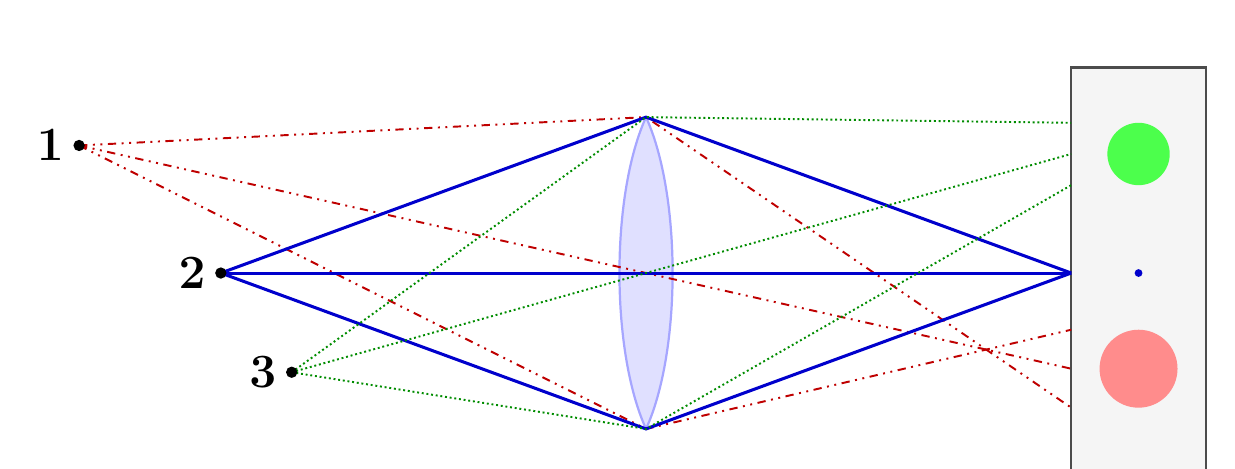
\begin{tikzpicture}[scale=0.9]
  % 像平面（右侧屏幕）
  \fill[gray!8] (6,-2.9) rectangle (7.9,2.9);
  \draw[black!70, line width=0.8pt] (6,-2.9) rectangle (7.9,2.9);

  % 双凸透镜
  \fill[blue!12]
      (0,2.2) .. controls (0.5,1.1) and (0.5,-1.1) .. (0,-2.2)
              .. controls (-0.5,-1.1) and (-0.5,1.1) .. (0,2.2);
  \draw[blue!35, line width=0.8pt]
      (0,2.2) .. controls (0.5,1.1) and (0.5,-1.1) .. (0,-2.2);
  \draw[blue!35, line width=0.8pt]
      (0,2.2) .. controls (-0.5,1.1) and (-0.5,-1.1) .. (0,-2.2);

  % 物点 1（远景，失焦）：暗红，点划线
  \draw[red!75!black, line width=0.7pt, dash dot dot] (-8,1.8) -- (0,2.2) -- (6,-1.9);
  \draw[red!75!black, line width=0.7pt, dash dot dot] (-8,1.8) -- (6,-1.35);
  \draw[red!75!black, line width=0.7pt, dash dot dot] (-8,1.8) -- (0,-2.2) -- (6,-0.8);

  % 物点 2（合焦）：蓝，实线，三条光线交于像平面上一点
  \draw[blue!80!black, line width=1.1pt] (-6,0) -- (0,2.2) -- (6,0);
  \draw[blue!80!black, line width=1.1pt] (-6,0) -- (6,0);
  \draw[blue!80!black, line width=1.1pt] (-6,0) -- (0,-2.2) -- (6,0);

  % 物点 3（近景，失焦）：绿，点线
  \draw[green!55!black, line width=0.7pt, densely dotted] (-5,-1.4) -- (0,2.2) -- (6,2.12);
  \draw[green!55!black, line width=0.7pt, densely dotted] (-5,-1.4) -- (6,1.68);
  \draw[green!55!black, line width=0.7pt, densely dotted] (-5,-1.4) -- (0,-2.2) -- (6,1.24);

  % 物点与标号
  \fill (-8,1.8) circle (0.08);
  \fill (-6,0) circle (0.08);
  \fill (-5,-1.4) circle (0.08);
  \node[left=2pt, font=\LARGE\bfseries] at (-8,1.8) {1};
  \node[left=2pt, font=\LARGE\bfseries] at (-6,0) {2};
  \node[left=2pt, font=\LARGE\bfseries] at (-5,-1.4) {3};

  % 像平面上的结果：中间合焦成点，上下两个是弥散圆
  \fill[green!70] (6.95,1.68) circle (0.44);
  \fill[blue!80!black] (6.95,0) circle (0.055);
  \fill[red!45] (6.95,-1.35) circle (0.55);
\end{tikzpicture}
\end{center}

景深（depth of field, DOF）定义为场景中看起来足够清晰（acceptably sharp）的最近物体与最远物体之间的距离。

控制景深的主要手段是光圈（aperture）大小：

\begin{itemize}
    \item 光圈越小，景深越大
    \item 但小光圈减少进光量，需要增加曝光时间，图像噪声更大
\end{itemize}

实际拍摄中的取舍是：大光圈适合拍摄孤立主体，例如夜景或人像；小光圈提供更大的景深，适合风景、流水等题材。

\subsection{Field of View}

视场（field of view, FoV）是相机所观测到的世界的角度范围。设传感器尺寸为 $d$，像距为 $z'$，视场角为 $\alpha$，则

\[
\tan\frac{\alpha}{2} = \frac{d/2}{z'}
\]

其中 $z' = (1+m)F$，$m$ 为放大率；对无穷远对焦时 $z' = F$。焦距越短，视场越大（广角）；焦距越长，视场越小（长焦）。
感受整体的风景效果，应当采用短焦镜头增大视角。拍摄远处的东西，采用长焦镜头。

\subsection{Lens Aberrations}

\subsubsection{Radial Distortion}

径向畸变（radial distortion）由透镜不完美引起，在广角镜头中尤其明显，越靠近图像边缘越显著，表现为图像内容被压缩。
负径向畸变指的是图像背离径向方向发生变形，这由于使用了超广角镜头，导致图片呈现木桶式的向外膨胀现象；正径向畸变反之，是向内陷入的现象。

建模时不再直接使用标准投影矩阵，而是分三步进行：

\begin{enumerate}
    \item 投影到“归一化”图像坐标（normalized image coordinates）：$x_n = x/z$，$y_n = y/z$
    \item 施加径向畸变：
    \[
    x_d = x_n\left(1 + k_1 r^2 + k_2 r^4\right), \qquad
    y_d = y_n\left(1 + k_1 r^2 + k_2 r^4\right)
    \]
    其中 $r^2 = x_n^2 + y_n^2$，$k_1, k_2$ 为畸变系数
    \item 施加焦距并平移到图像中心：$u = f x_d + c_x$，$v = f y_d + c_y$
\end{enumerate}

OpenCV 提供了标定和去畸变的实现。畸变对不同题材的影响不同：广角适合强调透视，标准镜头接近人眼观感，长焦则压缩空间。

\subsubsection{Chromatic Aberration}

玻璃的折射率随波长略有变化，因此简单透镜存在色差（chromatic aberration）：不同颜色的光聚焦在略微不同的距离上，表现为模糊和颜色偏移。为了减弱色差和其他像差，多数摄影镜头采用由不同玻璃元件（以及不同镀膜）组成的复合透镜（compound lens）。

\subsubsection{Vignetting}

湮灭，也叫暗角（vignetting），指亮度向图像边缘衰减的趋势。机械暗角（mechanical vignetting）是指光束的边缘部分被遮挡，从未到达像平面。这可能是由于使用两个透镜或者多个透镜的时候，光线通过了第一个透镜受到折射，没有通过第二个透镜从而导致边缘发生衰减。

\subsection{Colors}

\subsubsection{The Human Eye}

人眼与相机在结构上类似：虹膜（iris）相当于光圈，通过改变晶状体的形状对焦，视网膜（retina）相当于胶片或数字传感器。瞳孔（pupil）对应针孔或光圈，视网膜对应感光面。当眼睛正确对焦时，来自眼外物体的光被成像在视网膜上。

视网膜上有两种感光细胞：

\begin{itemize}
    \item \textbf{视杆细胞（rods）：}约 7500 万到 1.5 亿个，不参与颜色视觉，只提供灰度信息；灵敏度高，可以在夜间工作。
    \item \textbf{视锥细胞（cones）：}约 600 万到 700 万个，负责颜色视觉，在中等和高亮度条件下工作。视锥细胞有三种，光谱灵敏度峰值分别位于短波（S，420--440 nm）、中波（M，530--540 nm）和长波（L，560--580 nm）。
\end{itemize}

\subsubsection{CIE RGB}

由于人眼只有三种视锥细胞，原则上三个参数就足以描述任何一种人类颜色感觉。反过来，所有单色光（单一波长）都可以用三种适当选择的原色混合得到，即红（700.0 nm）、绿（546.1 nm）和蓝（435.8 nm）。

\subsection{Image Sensing}

\subsubsection{Imaging Pipeline}

从光到数字图像通常经过三个阶段：

\begin{enumerate}
    \item 相机镜头和机身中的物理光传输（physical light transport）
    \item 传感器芯片上的光子测量与转换（photon measurement and conversion）
    \item 图像信号处理（image signal processing, ISP）与图像压缩
\end{enumerate}

\begin{center}
\resizebox{\textwidth}{!}{%
\begin{tikzpicture}[
    font=\small,
    blk/.style={draw, fill=white, minimum height=1.15cm, text width=2.8cm,
                align=center, inner sep=2pt},
    grp/.style={draw, dashed, line width=0.7pt,
                fill={rgb,255:red,200;green,228;blue,246}},
    fl/.style={->, >=latex, line width=0.8pt},
    ln/.style={line width=0.8pt},
    cyl/.style={line width=0.8pt}
]

  % ================= 第一级：相机机身 =================
  \draw[grp] (0,1.1) rectangle (10.6,-2.3);
  \node[blk] (optics)   at (1.7,-0.35) {光学系统\\（Optics）};
  \node[blk] (aperture) at (5.1,-0.35) {光圈\\（Aperture）};
  \node[blk] (shutter)  at (8.5,-0.35) {快门\\（Shutter）};
  \draw[fl] (optics.east)   -- (aperture.west);
  \draw[fl] (aperture.east) -- (shutter.west);
  \node at (5.3,-1.85) {相机机身（Camera Body）};
  \node[align=center] at (-2.5,-0.35) {Scene\\Radiance};

  % ================= 第二级：传感器芯片 =================
  \draw[grp] (0,-3.0) rectangle (10.6,-6.4);
  \node[blk] (sensor) at (1.7,-4.5) {传感器\\（Sensor, CCD/CMOS）};
  \node[blk] (gain)   at (5.1,-4.5) {增益\\（Gain, ISO）};
  \node[blk] (adc)    at (8.5,-4.5) {模数转换\\（ADC）};
  \draw[fl] (sensor.east) -- (gain.west);
  \draw[fl] (gain.east)   -- (adc.west);
  \node at (5.3,-5.95) {传感器芯片（Sensor chip）};

  % ================= 第三级：图像信号处理器 =================
  \draw[grp] (0,-7.1) rectangle (10.6,-12.1);
  \node[blk] (demosaic) at (3.6,-8.1)  {去马赛克\\（Demosaic）};
  \node[blk] (denoise)  at (7.0,-8.1)  {去噪与锐化\\（Denoise and sharpen）};
  \draw[fl] (demosaic.east) -- (denoise.west);
  \node[blk] (wb)       at (1.7,-10.5) {白平衡\\（White Balance）};
  \node[blk] (gamma)    at (5.1,-10.5) {Gamma/曲线\\（Gamma/curve）};
  \node[blk] (compress) at (8.5,-10.5) {压缩\\（Compress）};
  \draw[fl] (wb.east)    -- (gamma.west);
  \draw[fl] (gamma.east) -- (compress.west);
  \node at (5.3,-11.65) {图像信号处理器（ISP）};

  % ================= 级间连线 =================
  % 相机机身 → 传感器芯片
  \draw[fl] (shutter.east) -- (11.8,-0.35) -- (11.8,-2.7) -- (-1.3,-2.7)
            -- (-1.3,-4.5) -- (sensor.west);

  % 传感器芯片 → RAW
  \draw[fl] (adc.east) -- (13.2,-4.5);

  % 传感器芯片 → 图像信号处理器
  \draw[fl] (11.8,-4.5) -- (11.8,-6.8) -- (-1.3,-6.8) -- (-1.3,-8.1)
            -- (demosaic.west);

  % 去噪与锐化 → 白平衡（ISP 内部回绕，绕行线在虚线框内）
  \draw[fl] (denoise.east) -- (10.0,-8.1) -- (10.0,-9.5) -- (0.6,-9.5)
            -- (0.6,-10.5) -- (wb.west);

  % 图像信号处理器 → JPEG
  \draw[fl] (compress.east) -- (13.2,-10.5);

  % ================= 输出：RAW / JPEG =================
  % RAW 数据库
  \fill[gray!25] (13.2,-3.7) -- (13.2,-5.3)
      arc[start angle=180, end angle=360, x radius=1.2, y radius=0.3]
      -- (15.6,-3.7) -- cycle;
  \draw[cyl] (13.2,-3.7) -- (13.2,-5.3)
      arc[start angle=180, end angle=360, x radius=1.2, y radius=0.3]
      -- (15.6,-3.7);
  \draw[cyl, fill=gray!45] (14.4,-3.7) ellipse (1.2 and 0.3);
  \node at (12.55,-4.2) {RAW};

  % JPEG 数据库
  \fill[gray!25] (13.2,-9.7) -- (13.2,-11.3)
      arc[start angle=180, end angle=360, x radius=1.2, y radius=0.3]
      -- (15.6,-9.7) -- cycle;
  \draw[cyl] (13.2,-9.7) -- (13.2,-11.3)
      arc[start angle=180, end angle=360, x radius=1.2, y radius=0.3]
      -- (15.6,-9.7);
  \draw[cyl, fill=gray!45] (14.4,-9.7) ellipse (1.2 and 0.3);
  \node at (12.55,-10.2) {JPEG};

\end{tikzpicture}%
}
\end{center}

\subsubsection{Shutter}

焦平面快门（focal plane shutter）位于图像传感器或胶片的正前方。多数数码相机使用机械快门与电子快门的组合。快门速度（即曝光时间）决定到达传感器的光量，进而决定图像是过曝、欠曝、模糊还是含噪。

\subsubsection{Sensor}

\begin{itemize}
    \item \textbf{CCD}：电荷在像素之间逐个移动，最终在输出节点统一转换为电压。
    \item \textbf{CMOS}：在每个像素内部完成电荷到电压的转换，目前是标准方案。
\end{itemize}

\subsubsection{Color Filter Array and Demosaicing}

为了测量颜色，像素按特定阵列排布，最常见的是 Bayer RGB 图案：每个 $2\times2$ 子块包含 2 个绿色、1 个蓝色和 1 个红色滤镜，每个滤镜覆盖一个像素传感器。这样每个像素只能测到一个通道，缺失的其他通道由邻域插值估计，这个过程称为去马赛克（demosaicing）。
一般的方法是在图像上进行双线性插值。

绿色滤镜占总数的一半，是因为人眼的亮度敏感函数（luminance sensitivity function）在绿色波段响应最强。

\subsubsection{Gamma Correction}

人眼对暗部区域的强度差异更加敏感，因此在离散化之前对强度或颜色做非线性变换是有利的，在读取时再撤销这一变换。通常取

\[
Y' = Y^{1/\gamma}
\]
这样可以给暗部留下更大的区间，最后离散化的时候梯度会更加细密，能够反映出更多细节，简而言之就是能用有限的空间牺牲一点“亮”和“很亮”的区别，保存“黑”和“灰的区别”。
同时早期的硬件输出的时候是非线性的，可以抵消一部分硬件问题。在当代，Gamma校正主要用于图像增强和特征值提取算法。

\subsection{Summary}

\begin{itemize}
    \item \textbf{相机：}针孔模型；世界坐标、相机坐标与图像坐标之间的变换；内参与外参；$3\times4$ 投影矩阵。
    \item \textbf{透镜：}透镜允许大孔径同时保持图像清晰；高斯透镜公式 $\frac{1}{f} = \frac{1}{z} + \frac{1}{z'}$。
    \item \textbf{景深：}由光圈控制，小光圈景深大但进光少、噪声大。
    \item \textbf{视场：}由传感器尺寸和像距决定，焦距越短视场越大。
    \item \textbf{畸变：}径向畸变、色差、暗角。
    \item \textbf{颜色与传感：}视杆与视锥细胞、CIE RGB、Bayer 阵列与去马赛克、Gamma 校正。
\end{itemize}

\section{Image Processing}

\subsection{Pixel (Point) Processing}

\subsubsection{Basic Pixel Operations}
Pixel Processing的基础操作主要有以下几个层面：

\begin{itemize}
    \item \textbf{变暗（darken）：}$I(x,y) - 128$
    \item \textbf{变亮（lighten）：}$I(x,y) + 128$
    \item \textbf{降低对比度（low contrast）：}$I(x,y)/2$
    \item \textbf{反色（invert）：}$255 - I(x,y)$
    \item \textbf{灰度化（gray）：}$\mathbf{dot}\bigl([0.3,\ 0.6,\ 0.1],\ I(x,y)\bigr)$，三个权重依次对应 R、G、B 通道，绿色权重最大
\end{itemize}

\subsubsection{Histogram Equalization}
Pixel Processing中较复杂的是直方图均衡化方法，用来调整图像中RGB通道的强度。用意在于调整比较复杂的颜色密度分布变换为均匀分布。这个方法的数学原理是将概率分布变换为均匀分布，寻找一个单调递增的映射函数T（为了保证是可逆的不丢失信息），将原有分布复合通过这个映射之后得到均匀分布。

具体的技巧是，首先把RGB的灰度分布曲线画出来（对每一个颜色通道，统计每种灰度对应的像素个数，然后归一化计算概率分布），得到概率密度函数pdf，积分得到cdf，将CDF的轴拉成255对应灰度值范围，然后将原始灰度数值映射为新的处理过后的灰度值。

\[
s_k = (L - 1)CDF(r_k)
\]

为什么CDF呢？论证的过程需要依照随机变量变换定理，变换的规则是变换前后在同一个足够小区间上的必须是一致的（概率总量守恒）

根据概率论中的随机变量变换定理，变量变换前后在区间 $[r, r+dr]$ 与 $[s, s+ds]$ 内的概率总量必须守恒：$$p_s(s) \vert{}ds\vert{} = p_r(r) \vert{}dr\vert{}$$

设原始图像的灰度值是一个连续随机变量 $r \in [0, L-1]$，其概率密度函数（PDF）为 $p_r(r)$。我们希望寻找一个单调递增的映射函数 $s = T(r)$，使得变换后的新灰度变量 $s$ 在 $[0, L-1]$ 上服从均匀分布，即：$$p_s(s) = \frac{1}{L-1}$$

由于映射函数 $T(r)$ 是单调递增的（以保证像素灰度相对大小顺序不颠倒，避免图像反色），有 $\frac{ds}{dr} > 0$，因此：$$p_s(s) = p_r(r) \cdot \frac{dr}{ds}$$3. 导出映射函数：累积分布函数（CDF）将要求的均匀分布 $p_s(s) = \frac{1}{L-1}$ 

代入上式：$$\frac{1}{L-1} = p_r(r) \cdot \frac{dr}{ds} \implies \frac{ds}{dr} = (L-1) p_r(r)$$对微分方程两边关于 $r$ 进行积分：$$s = T(r) = (L-1) \int_0^r p_r(w) \, dw = (L-1) \cdot F_r(r)$$其中 $F_r(r)$ 正是原始灰度的累积分布函数（CDF）。

值得注意的一个拓展：随机变量变换定理也可以倒过来用，C语言标准库中，使用标准随机数在y轴上面取值，反函数映射到x轴上，即可得到关于x的均匀随机分布。

\subsection{Filtering}

\subsubsection{Linear Filters}
\paragraph{Classification of Linear Filters}
图像滤波常常用于图像的模糊，锐化，特征提取等算法。线性滤波器就是根据不同的过滤原理实现卷积算子，是一个3*3的矩阵kernel，然后在图像周围补0,扫描整个图像。
\paragraph{Box Filter}
卷积核为全 1 矩阵除以元素个数，即邻域算术平均，得到低通模糊：
$$K_{\text{box}} = \frac{1}{9}\begin{bmatrix} 1 & 1 & 1 \\ 1 & 1 & 1 \\ 1 & 1 & 1 \end{bmatrix}$$

\paragraph{Gaussian Filter}
卷积核由二维高斯函数采样并归一化，中心权重大、四周小，同属低通滤波（Low Pass Filtering）：
$$K_{\text{gauss}} = \frac{1}{16}\begin{bmatrix} 1 & 2 & 1 \\ 2 & 4 & 2 \\ 1 & 2 & 1 \end{bmatrix}$$

\paragraph{Sharpening Filter}
单位冲激核减去均值核，得到高通核：
$$K_{\text{sharp}} = \begin{bmatrix} 0 & 0 & 0 \\ 0 & 2 & 0 \\ 0 & 0 & 0 \end{bmatrix} - \frac{1}{9}\begin{bmatrix} 1 & 1 & 1 \\ 1 & 1 & 1 \\ 1 & 1 & 1 \end{bmatrix}$$
等价于在原图上叠加被放大的高频成分：
$$\text{Sharpening: } I + \lambda\,(I - I_{\text{blur}})$$
其中 $I_{\text{blur}}$ 为低通滤波结果，$\lambda$ 为锐化强度系数。

\paragraph{Mathematical Background}
算法上来讲，为了实现高效的滤波，在Separable Filtering中采用数学技巧降低计算量。本质上在某些核中可以使用线性技巧，将矩阵Kernel展开到$K = vh^{T}$的形式，然后只需要做两个一维乘法。

线性滤波的数学特征主要有以下两个：

\begin{itemize}
    \item Correlation: $$g(i,j) = \sum_{k,l}f(i+k,j+l)h(k,l)$$
    \item Convolution: $$g(i,j) = \sum_{k,l}f(i-k,j-l)h(k,l)$$
\end{itemize}

这两个算子都具备线性和平移不变性。

\begin{itemize}
    \item $h \circ (f_0+f_1) = h \circ f_0 + h \circ f_1$
    \item Shift Invarience: $(h \circ g)(i , j) = (h \circ f)(i + h , j + l) $ 
\end{itemize}

Filter和卷积神经网络中的特征提取算法有非常紧密的联系。

\subsubsection{Non-linear Filters}

\paragraph{Bilateral Filter}

Gaussian滤波的主要困难在于只考虑了像素位置的相近性，但是没有考虑像素灰度的差异，会忽略边缘，让重要的信息变模糊。

将Gaussian滤波（Domain Kernel）和颜色（Range Kernel）变化的结合起来，得到Bilateral Filter的权重

\[
w (i,j,k,l) = \exp(-\frac{(i-k)^2+(j-l)^2}{2\sigma_{d}^{2}}-\frac{||f(i,j) - f(k,l)||^2}{2\sigma_{r}^{2}})
\]

将此作为权重，结合softmax的归一化操作，得到滤波核

\[
g(i,j) = \frac{f(k,l)w(i,j,k,l)}{w(i,j,k,l)} \Rightarrow softmax(-\frac{(F_i-F_j)^2}{\sigma}f)
\]

这种滤波技术常用于美颜磨皮和ps技术, 多模态学习中的Kernel本质上就是可以学习的滤波器。

\paragraph{Joint Bilateral Filter}

如果有高清图片作为参考，进行图像滤波的时候可以直接参照正确答案查看颜色的相似性，实现去噪（用没Flash的参照给有Flash的进行去噪）。这也是神经网络中自注意力的灵感来源。如果自身的颜色细节是不好的，滤波器中的sigma参数应当依据无Flash的高清图片来确定，得到joint滤波。

上图是 No-Flash 图某一行的灰度剖面，$\sigma_d$ 控制参与平均的空间邻近范围；下图是 Flash 图同一行的剖面，$\sigma_r'$ 由 Flash 图确定颜色相似范围。两者分别对应权重公式中的域核（Domain Kernel）与值核（Range Kernel）。

技术路径分三步：

\begin{enumerate}[label=\arabic*.]
    \item 以 Flash 图为引导图（guide），对 No-Flash 图做 Joint Bilateral Filter，得到去噪后的基础层：
    \[
    I_{\mathrm{base}} = \mathrm{JBF}(I_{\mathrm{noflash}} \mid I_{\mathrm{flash}})
    \]
    \item 对 Flash 图做普通 Bilateral Filter 得到其平滑版本，再相除提取细节层：
    \[
    I_{\mathrm{detail}} = I_{\mathrm{flash}} / \mathrm{BF}(I_{\mathrm{flash}})
    \]
    \item 两者相乘，把 Flash 图的高频细节搬回低噪声的 No-Flash 图上：
    \[
    I_{\mathrm{result}} = I_{\mathrm{base}} \times I_{\mathrm{detail}}
    \]
\end{enumerate}

想要保持细节，则可以对原图进行滤波，提取高频细节。高频细节为了得到对比度，原图不带闪光灯饱和度低，对比时不宜使用减法提取，应该用除法提取对比度高的图像。

\subsection{UpSampling \& DownSampling}

\subsubsection{DownSampling and Anti-aliasing}
减小图像尺寸如果要通过降采样随机丢弃行列的方法进行实现，有可能出现走样的情况。这是因为采样频率无法反映图形中的高频噪声和高频细节，所以出现了不知所谓的结果。解决的方法是首先进行高斯滤波，将图像变得平滑。

将高斯平滑的方法和sampling排列起来，则可以构造出Gaussian金字塔，表现这个缩小的过程。

\begin{figure}[H]
    \centering
    \includegraphics[width=0.9\textwidth]{/home/simson/图片/截图/截图 2026-09-24 10-27-33.png}
    \caption{Gaussian 金字塔：每一级先做高斯模糊（Blur）再降采样（Subsample），逐级得到尺寸减半的图像}
\end{figure}

\paragraph{Laplacian Pyramid}

高斯金字塔每一级只保留低通信息，细节在模糊与降采样中被丢掉了。把相邻两级相减，就能把这些细节显式地取出来：

\[
L_i = G_i - \text{upsample}(G_{i+1}), \qquad G_i = L_i + \text{upsample}(G_{i+1})
\]

其中 $\text{upsample}(\cdot)$ 就是下一小节的插值放大（对应图中的 ``$\times 2$'' 节点），相减对应图中的圆圈；最粗的一级没有更粗的层可减，直接取 $L_4=G_4$。

\begin{figure}[ht]
    \centering
    \includegraphics[width=0.82\textwidth]{/home/simson/图片/截图/截图 2026-09-24 10-32-55.png}
    \caption{Laplacian 金字塔：$L_i$ 是 $G_i$ 减去放大后的 $G_{i+1}$ 所得的残差}
\end{figure}

右式说明这个表示是\textbf{可逆}的：从 $L_4$ 逐层加回去即可无损重建原图，而单用高斯金字塔则只有低通信息。$\{L_1,\dots,L_4\}$ 的优势可以顺着图看：

\begin{itemize}
    \item \textbf{分辨率分层}：$L_1$ 是最细的纹理与边缘，$L_2$、$L_3$ 依次是更粗的结构，$L_4$ 是那张最小的图，基本只剩低频。每一层对应一个明确的尺度，可以单独处理。
    \item \textbf{分频带（band-pass）}：每层只保留相邻两个尺度之间那一带频率。图中 $L_1$、$L_2$ 呈灰底加少量纹理，说明带通系数大多接近 0、非常稀疏，量化、阈值化和压缩都很划算（拉普拉斯金字塔是早期图像压缩的方案，也是小波变换的前身）。
    \item \textbf{冗余很小}：每层样本数按 $1/4$ 递减，加总约为原图的 $4/3$，只多花三分之一的空间就换来多尺度表示。
    \item \textbf{便于分尺度编辑}：亮度和细节被拆到了不同层，做色调映射、细节增强时可以只动某一层而不波及其他尺度；做图像融合时在不同层分别加权，还能避免拼接处的接缝。
\end{itemize}

图中每个 ``$\times 2$'' 节点都要靠插值把粗层放大来\textbf{预测}细层，预测得越准，残差层就越稀疏、越好压缩——这正是保边上采样（如 JBU）在实践中的价值。
Laplacian 金字塔因为逐级分频率保存信息，可以在数据传输中实现逐渐叠加，从模糊到清晰的效果。同时可以作为一种可以恢复原状的图像压缩技术。

下面总结并阐述了Laplacian金字塔的构造过程和处理流程：

\begin{figure}[H]
    \centering
    \includegraphics[width=0.70\textwidth]{/home/simson/图片/截图/截图 2026-09-24 10-41-19.png}
    \caption{Laplacian 金字塔的分解（左）与重建（右）流程}
\end{figure}

左半是分解：每级先用高斯滤波 $H_0$ 平滑、再降采样 $\downarrow 2$ 得到粗层，粗层经上采样 $\uparrow 2$ 与插值 $I$ 回到细层网格后，在求和点与原图相减（$-$）得到该级的细节残差，再进入下一级，如此逐级级联；右半是重建：各层数据经 $Q$ 后逐级上采样、插值并相加，最终得到输出 $O$。黄色块是各层的图像数据，蓝色块是可逆的滤波算子。

\paragraph{Mathematics of the Laplacian Pyramid}

根据构造流程，首先进行Gauss滤波，然后将不同程度的Gauss滤波进行做差和求微分过程：

\[
G(x, y ,\sigma) = \frac{1}{2 \pi \sigma} e ^{-\frac{x ^ 2 + y ^ 2}{2 \sigma^2}} \qquad \nabla^2 f = \frac{\partial^2 f}{\partial x ^ 2} + \frac{\partial^2 f}{\partial y^2}
\]

根据上述函数，将laplace算子作用在上面。

\[
\nabla^2 G(x , y ,\sigma) = (\frac{x ^ 2 + y ^ 2}{\sigma^4} - \frac{2}{\sigma^2})G(x, y, \sigma) = \frac{\partial G}{\partial \sigma} \frac{1}{\sigma}
\]

得到了Gauss函数非常重要的数学关系，使用展开式进行离散化。

\[
\sigma \nabla^2 G(x, y, \sigma) = \frac{\partial G}{\partial \sigma} \simeq (\frac{G(x,y,h\sigma) - G(x,y,\sigma)}{k\sigma - \sigma})
\]

化简得到：

\[
G(x, y ,k\sigma) - G(x, y, \sigma) \simeq (k-1)\sigma^2 \nabla^2 G
\]

这就是laplace金字塔的数学模型。

\subsubsection{UpSampling}

把小的图片放大，会出现非常模糊的情况，为了避免简单使用放大像素的方法，需要进行插值。

插值的数学原理可以用如下公式进行表示，以一元函数插值为例：

设采样点为整数位置 $x_k$，已知采样值 $f(x_k)$，插值即构造 $g(x)$ 满足 $g(x_k)=f(x_k)$，并用于估计采样点之间的函数值。记 $x$ 落在区间 $[x_k,x_{k+1}]$ 内，$t=x-x_k\in[0,1)$。

最近邻插值（Nearest Neighbor）：取离 $x$ 最近的采样值，$g(x)$ 是阶梯函数
\[
g(x)=f(x_k),\qquad k=\arg\min_{j}|x-x_j|
\]

线性插值（Linear）：用相邻两点连直线
\[
g(x)=(1-t)\,f(x_k)+t\,f(x_{k+1})
\]

Cubic 插值：在每个区间上用三次多项式，由两端函数值与一阶导数连续共四个条件定出系数
\[
g(x)\big|_{[x_k,x_{k+1}]}=a_3(x-x_k)^3+a_2(x-x_k)^2+a_1(x-x_k)+a_0
\]
\[
g(x_k)=f(x_k),\quad g(x_{k+1})=f(x_{k+1}),\quad g'(x_k^-)=g'(x_k^+),\quad g'(x_{k+1}^-)=g'(x_{k+1}^+)
\]

插值的方法有最近邻插值法，线性插值法。最近邻插值就是直接把最近邻居的数值搬过来，形成类似直方图的函数状态；比这个效果稍好的是线性插值，可以至少具有丰富的变化和导数。效果更好的是选取分段的高次函数，比如Cubic插值选用三次函数保证一阶连续。

放到图像上采样的插值算法中，双线性插值法是较为常用的，只需要知道周围四个邻居的数值，但是注意，双线性插值是一种非线性插值，结果中有交叉项。如果要追求好的效果，用Bicubic插值。

双线性插值（Bilinear）：用周围四个邻居。记 $u=x-i,\ v=y-j$，$(u,v)\in[0,1)^2$
\[
g(x,y)=(1-u)(1-v)f(i,j)+u(1-v)f(i+1,j)+(1-u)v\,f(i,j+1)+uv\,f(i+1,j+1)
\]
写成矩阵形式，交叉项 $uv$ 出现在展开后的二次项中：
\[
g(x,y)=
\begin{bmatrix}1-u & u\end{bmatrix}
\begin{bmatrix}f(i,j) & f(i,j+1)\\ f(i+1,j) & f(i+1,j+1)\end{bmatrix}
\begin{bmatrix}1-v\\ v\end{bmatrix}
\]

Bicubic 插值：用周围 $4\times4=16$ 个邻居，两个方向分别套用同一个三次核 $W$，可分离地写成
\[
g(x,y)=\sum_{m=-1}^{2}\sum_{n=-1}^{2} f(i+m,\ j+n)\,W(u-m)\,W(v-n)
\]
其中 $W$ 为三次卷积核（$a$ 通常取 $-0.5$）
\[
W(s)=
\begin{cases}
(a+2)|s|^3-(a+3)|s|^2+1, & |s|\le 1\\[2pt]
a|s|^3-5a|s|^2+8a|s|-4a, & 1<|s|<2\\[2pt]
0, & |s|\ge 2
\end{cases}
\]

\subsubsection{Joint Bilateral Upsampling}

\paragraph{Motivation: Why Upsample Jointly}

深度估计（立体匹配 stereo matching、多视图立体 multi-view stereo 等）需要为每个像素在一系列候选视差（disparity）上做匹配，代价随像素数增长，通常是整个流程中最贵的一步。如果最终只需要一张低分辨率的深度图，一个常见的加速方案是把流程拆成三步：

\begin{enumerate}[label=\arabic*.]
    \item 对输入图像降采样（downsample），得到低分辨率彩色图；
    \item 在低分辨率上估计深度图（estimate the depth image）；
    \item 把深度图上采样（upsample）回原始分辨率。
\end{enumerate}

前两步的代价大致与像素数成正比，因此把最贵的深度估计放到低分辨率上做，代价可以显著下降，这就是 ``for significant speedup'' 的含义。问题出在第三步：直接用上一节的最近邻、双线性或 Bicubic 插值放大深度图，并不能得到满意的结果。这些插值只关心样本之间的空间距离，完全不知道图像内容；而深度图在物体边界处存在跳变（discontinuity），插值核会把边界两侧的样本一起平均，于是边界被抹成一条斜坡，与真实的三维结构不符。最近邻插值虽然不会模糊，但会产生块状锯齿。

\begin{figure}[H]
    \centering
    \includegraphics[width=0.95\textwidth]{/home/simson/图片/截图/截图 2026-09-24 10-20-31.png}
    \caption{联合双边上采样的动机：降采样—估计深度—上采样，上采样时复用原始输入图像的边缘信息}
\end{figure}

于是自然的想法是：不要只在深度图内部插值，而是\textbf{复用原始输入图像中的边缘信息}（reuse the edge information in the original input image）。物体的边界在彩色图和深度图上出现在同一位置，高分辨率彩色图仍然保留着低分辨率深度图已经丢失的边界位置，因此可以把它作为引导图（guide），让插值权重在颜色发生跳变的地方被截断。

\paragraph{The JBU Formula}

Kopf 等人把上一节双边滤波的思想搬到上采样任务上，提出了联合双边上采样（Joint Bilateral Upsampling, JBU）。设低分辨率深度图为 $S$，高分辨率彩色引导图为 $\tilde I$，则高分辨率深度图上像素 $p$ 的取值为

\[
\tilde S_p = \frac{1}{k_p}\sum_{q_\downarrow\in\Omega} S_{q_\downarrow}\ f(\|p_\downarrow - q_\downarrow\|)\ g(\|\tilde I_p - \tilde I_q\|)
\]

其中各符号的含义为：

\begin{itemize}
    \item $p$：高分辨率输出图上的目标像素；$p_\downarrow$ 是它在低分辨率网格上的对应坐标（$\downarrow$ 表示低分辨率深度图中的坐标）。
    \item $q_\downarrow$：低分辨率深度图中落在 $p_\downarrow$ 邻域 $\Omega$ 内的样本点，求和遍历整个 $\Omega$。
    \item $S_{q_\downarrow}$：该样本点的低分辨率深度值，也就是被插值的信号。
    \item $\tilde I_p,\tilde I_q$：高分辨率彩色引导图在对应位置的取值。
    \item $f$ 与 $g$ 都是高斯函数（Gaussian function）：$f$ 作用在空间距离上，是域核（domain kernel）；$g$ 作用在颜色差上，是值核（range kernel）。
    \item $k_p$：归一化因子（normalization factor），即所有权重之和 $k_p=\sum_{q_\downarrow\in\Omega} f\,g$，使权重归一化到和为 1。
\end{itemize}

公式的结构与双边滤波完全一致，区别集中在两点：

\begin{itemize}
    \item 空间项 $f$ 是在\textbf{低分辨率}坐标上计算的，$\|p_\downarrow-q_\downarrow\|$ 度量的是样本到目标位置的距离。它扮演插值核的角色：距离越远权重越小，从而在稀疏的低分辨率样本之间平滑地重建出高分辨率的取值。
    \item 颜色项 $g$ 取的是\textbf{高分辨率}彩色图。当样本跨过物体边界时，$\|\tilde I_p-\tilde I_q\|$ 很大，$g$ 迅速趋近于 0，跨越边界的样本被排除在平均之外。
\end{itemize}

因此 $f$ 负责“插值”（保持平滑），$g$ 负责“保边”（在颜色跳变处截断），二者相乘得到一个形状随位置变化、由引导图决定的插值核。这正是它比固定核的 Bicubic 插值更贴合真实边界的原因。

\begin{figure}[H]
    \centering
    \includegraphics[width=0.95\textwidth]{/home/simson/图片/截图/截图 2026-09-24 10-22-53.png}
    \caption{联合双边上采样在一维信号上的过程：左列为信号（上：低分辨率深度；下：高分辨率彩色），中列为两个高斯权重 $f$、$g$，右列为相乘后的权重与上采样结果 $\tilde S_p$}
\end{figure}

上图把公式在一维信号上逐步展开。第一行是空间部分：低分辨率深度图在边界处有一个跳变，目标位置 $p$ 用蓝色星号标出，落在低的那个台阶上；空间权重 $f$ 是以 $p_\downarrow$ 为中心的高斯；它与信号相乘后，在低分辨率样本上得到一条以 $p$ 为中心的权重曲线。第二行是颜色部分：高分辨率彩色图在对应位置也有一个跳变，颜色权重 $g$ 在颜色与 $\tilde I_p$ 相同的区域接近 1，一跨过边界就掉到 0；于是把 $f$ 与 $g$ 相乘得到的组合权重中，位于边界另一侧的样本权重被压制为 0。最终结果是高分辨率深度图 $\tilde S_p$：既在物体内部平滑，又保持了锐利的边界，而且边界位置正好落在彩色图的边缘上。

\paragraph{Comparison with Other Upsampling Methods}

\begin{figure}[H]
    \centering
    \includegraphics[width=0.95\textwidth]{/home/simson/图片/截图/截图 2026-09-24 10-23-07.png}
    \caption{四种上采样方法在深度图边界处的对比（上排为放大的深度图区域，下排为对应的高分辨率彩色图）}
\end{figure}

同一张低分辨率深度图用四种方法放大，效果差别很明显：

\begin{itemize}
    \item \textbf{最近邻上采样（Nearest Neighbor）}：直接复制最近样本，深度值不产生新的中间值，但边界走样成块状的锯齿，呈阶梯状；
    \item \textbf{双线性 / Bicubic 上采样}：结果平滑，但深度边界被抹成一条逐渐过渡的斜坡，与彩色图中的锐利边缘不再对齐；
    \item \textbf{高斯上采样（Gaussian）}：本质上是各向同性的低通插值，模糊更严重，边界更加弥散；
    \item \textbf{联合双边上采样（JBU）}：在物体内部平滑过渡，在边界处与彩色图的边缘对齐，得到既连续又锐利的深度图。
\end{itemize}

\paragraph{Discussion}

\begin{itemize}
    \item 与上一节的联合双边滤波相比，这里的“联合”体现在两个不同分辨率的信号上：被滤波的是低分辨率深度图，提供颜色相似性判据的却是高分辨率彩色图。若引导图就是被滤波图像本身、且两者分辨率相同，公式即退化为普通的双边滤波。
    \item 计算上，每个高分辨率像素只需要遍历一个小邻域 $\Omega$（例如 $4\times 4$ 个低分辨率样本），比直接在高分辨率上重新估计深度便宜得多，因此适合作为“低分辨率估计 + 高分辨率恢复”这一套流程的最后一步。
    \item 这种用引导图决定滤波核形状的思路后来被推广为引导滤波（Guided Filter）等边缘保持滤波方法，也常出现在深度图增强、深度上采样以及需要从低分辨率标注恢复高分辨率预测的任务中。
\end{itemize}

Kopf, Johannes, et al. ``Joint bilateral upsampling.'' \textit{ACM Transactions on Graphics}, 2007.

\subsubsection{Image Blending}

这是Laplacian金字塔在图像混合中的重要应用。图像混合要让低频的噪声尽可能均匀混合，同时体现出高频部分的线条，物体等等，laplace金字塔可以分开不同的频率，因此常常被用在类似的操作中。

具体做法分四步：

\begin{enumerate}[label=\arabic*.]
    \item 对两张源图分别建立 Laplacian 金字塔 $\{L_i^{A}\}$、$\{L_i^{B}\}$；
    \item 对掩膜 $M$ 建立 Gaussian 金字塔 $\{M_i\}$，逐级模糊相当于逐级加宽过渡带；
    \item 在每一层分别混合 $L_i = M_i \odot L_i^{A} + (1-M_i)\odot L_i^{B}$；
    \item 把混合后的各层折叠（collapse，逐级上采样并相加）回一张图像。
\end{enumerate}

\begin{figure}[H]
    \centering
    \includegraphics[width=0.72\textwidth]{/home/simson/图片/截图/截图 2026-09-24 11-04-41.png}
    \caption{Laplacian 金字塔融合：每一行是一个频带，两张图在该频带上按掩膜加权相加，最后把所有频带折叠回图像}
\end{figure}

图中每一行就是一个频带，自上而下由细到粗：最上面一行是最细的高频带，掩膜几乎还是硬边；越往下频带越粗，掩膜被模糊得越厉害，最下面一行只剩大范围的平滑过渡，混合的主要是颜色与亮度。这正是图中 Key Idea 的含义——``blend lower frequency bands over larger spatial ranges, high frequency bands over small spatial ranges''：低频用大范围过渡，所以看不到接缝；高频用小范围过渡，所以纹理和边缘不会被糊掉。直接按掩膜逐像素加权会在边界留下可见的接缝，而先把掩膜模糊又会连带糊掉细节，金字塔融合用“过渡带宽度随频带变化”同时避开了这两个问题。

这也点出了金字塔表示的价值：同一个边界在不同频带上需要不同的空间尺度，只有先把图像拆成频带，才可能对它们分别处理（Burt \& Adelson, 1983）。

\subsection{Image Transformation}

\paragraph{Image Warping}

Image Warping指的是对图像的几何变形，比如旋转，伸缩，拉伸，变形等等。要点在于如果直接映射原来图像到新图像，则会出现空洞或重叠现象。重点方法在于扫描目标图像，逆映射到原图的实数值，然后通过插值方法取得像素的数值，保证不会重复计算，全面覆盖。

\begin{figure}[H]
    \centering
    \includegraphics[width=0.75\textwidth]{/home/simson/图片/截图/截图 2026-09-24 11-23-04.png}
    \caption{反向映射：对目标图的每个像素 $x'$ 用逆映射求出源位置 $x=\hat h(x')$，再在源图上重采样}
\end{figure}

对目标图像 $g(x')$ 中的每一个像素：

\begin{enumerate}[label=\arabic*.]
    \item 用逆映射 $\hat h$ 算出它在源图中的位置 $x=\hat h(x')$；
    \item 在源图 $f$ 的该位置重采样（resample），把结果复制到 $g(x')$。
\end{enumerate}

两个实现细节：

\begin{itemize}
    \item $\hat h$ 是 $h$ 的逆映射。如果反过来遍历源像素、算出目标位置再写过去，目标图上会出现空洞（相邻源像素被拉开）与重叠（多个源像素落到同一格）；反向映射则保证每个目标像素恰好被写入一次。
    \item 重采样用双线性插值：$\hat h(x')$ 通常不是整数坐标（图中下排的红点落在四个格点之间），需要由它周围四个源像素加权得到取值，也就是 3.3.2 节讲的双线性插值。
\end{itemize}

\paragraph{Image Morphing}

Image Morphing指的是两个图像进行融合叠加的方法，实质上是分块的Warping和blending。

Morphing 的具体步骤（源图 $s$、目标图 $u$，进度参数 $\mu\in[0,1]$）：

\begin{enumerate}[label=\arabic*.]
    \item 在两幅图上选取一一对应的特征点（feature points），各自做 Delaunay 三角剖分，得到网格 $T_s$、$T_u$；
    \item 对三角形的位置做线性插值，得到中间网格 $T = \mu T_s + (1-\mu) T_u$；
    \item 按 $T_s \to T$ 与 $T_u \to T$ 的对应关系，在每个三角形内把两幅图分别 warp 成 $\tilde s$、$\tilde u$（三角形内部的映射由三个顶点唯一确定，是仿射变换）；
    \item 把两幅已经对齐的图像按颜色混合，输出 $o = \mu\tilde s + (1-\mu)\tilde u$。
\end{enumerate}

\begin{figure}[H]
    \centering
    \includegraphics[width=0.75\textwidth]{/home/simson/图片/截图/截图 2026-09-24 11-23-21.png}
    \caption{Image morphing：$T_s$、$T_u$ 是源图与目标图的 Delaunay 三角剖分，插值出中间网格后在每个三角形内 warp 并混合}
\end{figure}

$\mu$ 由 0 变到 1 时，输出的几何形状与颜色同时从源图过渡到目标图：前者靠 warping，后者靠 cross-dissolve（线性混合），morphing 正是两者的组合。

\section{Figure Detection}

\subsection{Edge Detection}

\paragraph{Mathematical Principle and Matrix Discretization}

边缘是图像中亮度发生突变（不连续）之处：表面法向、深度、颜色、光照的不连续都会形成边缘，而边缘携带了图像中大部分语义与形状信息，因此它是最先被提取的特征。数学上把灰度图视作二维函数 $f(x,y)$，"突变"就是函数在某处变化剧烈，用导数来度量。把沿 $x$、$y$ 的偏导数堆叠起来即得梯度
\[
\nabla f=\begin{bmatrix} f_x \\ f_y \end{bmatrix}
=\begin{bmatrix} \partial f/\partial x \\ \partial f/\partial y \end{bmatrix},
\qquad
|\nabla f|=\sqrt{f_x^2+f_y^2},
\qquad
\theta=\arctan\frac{f_y}{f_x}.
\]
在一维剖面上，边缘正对应一阶导数的极值；到二维就是梯度幅值 $|\nabla f|$ 的大值，$\theta$ 给出边缘的法向。

图像是离散采样的，导数只能由差商近似。从泰勒展开 $f(x+h)=f(x)+f'(x)h+\frac{f''(x)}{2!}h^2+\cdots$ 出发，取 $h=1$ 得前向差分 $f_x\approx f(x+1,y)-f(x,y)$；若把 $x+1$ 与 $x-1$ 两处的展开相减，二阶项相消，得到中心差分
\[
f_x\approx\frac{f(x+1,y)-f(x-1,y)}{2},
\]
它一步就有 $O(h^2)$ 精度（前向差分只有 $O(h)$），因此实际中一律采用中心差分。

真正让导数能在计算机上"跑起来"的是矩阵离散化：差商不过是相邻像素的加权和，因而可以写成一个卷积核。一维情形是 $[-1\ \ 1]$（前向）与 $[-1\ \ 0\ \ 1]$（中心）；二维时把一维核沿另一方向复制，再叠加平滑权，就得到
\[
H_x^{\text{Prewitt}}=\begin{bmatrix}-1&0&1\\-1&0&1\\-1&0&1\end{bmatrix},\quad
H_y^{\text{Prewitt}}=\begin{bmatrix}1&1&1\\0&0&0\\-1&-1&-1\end{bmatrix},
\]
\[
H_x^{\text{Sobel}}=\begin{bmatrix}-1&0&1\\-2&0&2\\-1&0&1\end{bmatrix},\quad
H_y^{\text{Sobel}}=\begin{bmatrix}1&2&1\\0&0&0\\-1&-2&-1\end{bmatrix}.
\]
于是求导退化为 3.2 节讲过的卷积滤波：$f_x=f*H_x$，$f_y=f*H_y$。核中的 $\pm1$ 在做差商、$0$ 在取中心、权重 $2$ 与 $1$ 在做平滑——Prewitt 与 Sobel 的唯一差别就在平滑权：Sobel 把中间行加倍，相当于在求导方向上再叠一个 $[1,2,1]$ 的二项式核，对噪声更稳健。

\begin{figure}[H]
    \centering
    
\includegraphics[width=0.85\textwidth]{/home/simson/latex/CSAI note/CV/figs/edge-prewitt-sobel-kernels.png}
    \caption{Prewitt 与 Sobel 的导数核：水平核（对 $x$ 求导）与垂直核（对 $y$ 求导）都是 3$\times$3 矩阵，即离散化后的偏导算子}
\end{figure}

把 $|\nabla f|$ 阈值化即可得到边缘图（Sobel 边缘检测器），但阈值很脆弱、很难选：偏高会漏掉弱边缘，偏低又会把噪声当成边缘——这正是后面 Canny 用非极大值抑制与双阈值要解决的问题。

\paragraph{Noise Suppression and the Gaussian Derivative}

噪声对导数是致命的。设观测图像为 $I_{i,j}=T_{i,j}+\epsilon_{i,j}$，其中 $T$ 是真实图像，$\epsilon_{i,j}\sim N(0,\sigma^2)$ 是各像素独立同分布的噪声。用中心差分求导时，噪声被一并相减：
\[
D_{i,j}=(T_{i,j+1}+\epsilon_{i,j+1})-(T_{i,j-1}+\epsilon_{i,j-1})
=(T_{i,j+1}-T_{i,j-1})+(\epsilon_{i,j+1}-\epsilon_{i,j-1}).
\]
后一项是两个独立高斯之差，仍是高斯，但方差相加：$\epsilon_{i,j}-\epsilon_{k,l}\sim N(0,2\sigma^2)$，即\textbf{方差翻倍}，标准差被放大 $\sqrt2$ 倍。平坦区域里真实差分近似为零，导数图便由纯噪声主导，真正的边缘被完全淹没。

解决办法是"先平滑、再求导"：先用高斯核 $g$ 平滑图像再做微分，即求 $\frac{d}{dx}(f*g)$。由卷积与微分可交换，
\[
\frac{d}{dx}(f*g)=f*\frac{dg}{dx},
\]
所以两趟卷积能合并成一趟：只需先把高斯核求导得到"高斯导数"核 $\frac{dg}{dx}$（一维上是一侧为正、一侧为负的反对称波形），再与图像卷积一次，就同时完成了去噪与求导。二维下对应两个核 $G_x=\partial G_\sigma/\partial x$ 与 $G_y=\partial G_\sigma/\partial y$，按网格离散化就是对采样点直接求偏导：
\[
G_x[i,j]=-\frac{i}{\sigma^2}e^{-\frac{i^2+j^2}{2\sigma^2}},\qquad
G_y[i,j]=-\frac{j}{\sigma^2}e^{-\frac{i^2+j^2}{2\sigma^2}},
\]
于是 $f_x=f*G_x$、$f_y=f*G_y$，一个水平、一个垂直。

\begin{figure}[H]
    \centering
    
\includegraphics[width=0.95\textwidth]{/home/simson/latex/CSAI note/CV/figs/gaussian-derivative-1d.png}
    \caption{高斯导数：$\frac{d}{dx}(f*g)=f*\frac{dg}{dx}$ 把去噪与求导合并为一趟卷积；右侧是二维的 $\frac{\partial G_\sigma}{\partial x}$ 与 $\frac{\partial G_\sigma}{\partial y}$}
\end{figure}

代价是尺度上的两难：$\sigma$ 越大去噪越彻底，但边缘同时被抹平，导数峰展宽、定位精度下降（课件分别用 1、3、7 像素的高斯核：越小噪声残留越多，越大边缘越糊）。"去噪"与"保边定位"无法兼得，$\sigma$ 只能折中——这也解释了为什么 Canny 的第一步（灰度化 + 高斯滤波）与 Harris 角点的预处理都要先做高斯平滑。

\paragraph{Canny Edge Detector}

Canny 检测器把前面几节的工具串成一条六步流水线，目标是得到"细、连续、定位准"的边缘：

\begin{enumerate}[label=\arabic*.]
    \item \textbf{预处理：灰度化 + 高斯模糊}。先把彩色图转成灰度图（边缘本是由亮度突变定义的），再用高斯核平滑以抑制噪声——这正是上一段的动机：求导会放大噪声，所以必须先平滑。
    \item \textbf{中心差分求梯度图}。用 Sobel 的中心差分算出 $G_x$、$G_y$（而不用前向差分，因为中心差分精度更高）。$G_x$ 突出竖直边缘、$G_y$ 突出水平边缘。
    \item \textbf{计算梯度幅值}。$|\nabla f|=\sqrt{G_x^2+G_y^2}$，即边缘强度图。
    \item \textbf{非极大值抑制（Non-Maximum Suppression）}。幅值图上的边缘是粗的：边缘附近一整条带上的像素幅值都很大。做法是遍历幅值矩阵，只保留沿\textbf{梯度方向}的局部极大值。对像素 $q$，沿梯度方向取它两侧的邻居 $p$ 与 $r$；梯度方向一般不落在整数格点上，故 $r$ 由相邻两点线性插值得到 $r=\alpha b+(1-\alpha)a$。当且仅当 $q>p$ 且 $q>r$ 时保留 $q$，否则置零——一条粗边就被削成单像素宽。
    \item \textbf{双阈值}。设高阈值（如 $0.7$）与低阈值（如 $0.3$）：高于高阈值的像素确定是边缘（强边缘），低于低阈值的一定不是，介于两者之间的是\textbf{弱边缘}，留给下一步判定。用双阈值取代单阈值，正是为了化解上一段末尾说的"阈值难选"：单阈值偏高会漏掉弱边缘，偏低又会引入噪声。
    \item \textbf{滞后边缘跟踪（Edge Tracking by Hysteresis）}。与强边缘相连的弱边缘判为真实边缘而保留，不与任何强边缘相连的弱边缘则丢弃。这一步让边缘在弱对比处仍能连续延伸，同时排除孤立的噪声响应。
\end{enumerate}

\begin{figure}[H]
    \centering
    
\includegraphics[width=0.95\textwidth]{/home/simson/latex/CSAI note/CV/figs/canny-non-maximum-suppression.png}
    \caption{非极大值抑制：沿梯度方向比较 $q$ 与两侧的 $p$、$r$（$r$ 由 $a$、$b$ 线性插值），只保留局部极大值，把粗边缘削成单像素宽}
\end{figure}

\paragraph{Applications of the Canny Detector}

Canny 给出的单像素、连续的边缘图本身就是物体的"线稿"，因此常被当作下游任务的条件输入：

\begin{itemize}
    \item \textbf{草图生成与三维形状生成}。Locally Attentional SDF Diffusion for Controllable 3D Shape Generation（SIGGRAPH 2023）用 Canny 从渲染图中提取线稿，再以线稿为条件生成可控的三维形状。
    \item \textbf{文本到图像的附加控制}。Adding Conditional Control to Text-to-Image Diffusion Models 中用 Canny 边缘图作为空间条件注入扩散模型，于是"一张线稿 + 一句文本描述"就能精确控制生成图像的构图。
    \item \textbf{通用轮廓提取}。图像编辑的选区引导、工业检测的缺陷轮廓、多视图几何中的特征线提取等，都把 Canny 当作默认的边缘算子。
\end{itemize}

\begin{figure}[H]
    \centering
    
\includegraphics[width=0.95\textwidth]{/home/simson/latex/CSAI note/CV/figs/canny-application-sketch3d.png}
    \caption{应用一：用 Canny 从渲染图提取线稿，作为三维形状生成的可控条件（Locally Attentional SDF Diffusion, SIGGRAPH 2023）}
\end{figure}

\begin{figure}[H]
    \centering
    
\includegraphics[width=0.95\textwidth]{/home/simson/latex/CSAI note/CV/figs/canny-application-controlnet.png}
    \caption{应用二：Canny 线稿作为扩散模型的空间控制条件，同一张线稿配不同文本可生成不同风格的图像（ControlNet / Adding Conditional Control to Text-to-Image Diffusion Models）}
\end{figure}

不过课件最后提醒：\textbf{边缘检测至今仍是一个未解决的问题}。人眼能把图中的物体轮廓干净地分割出来，而梯度幅值图在物体内部与背景处的杂散响应同样强烈，二者相差甚远。这也正是接下来要从边缘转向更能刻画局部结构的特征——角点与 blob——的原因。

\end{document}
